% Lecture Template for ME3050-001-002-Tristan Hill - Spring 2020 - Summer 2020
% Dynamics Modeling and Controls
% Second Order Time Response - Topic 3

% I am finally converting my stuff to BEAMER

% Document settings

%\documentclass{beamer}          % for presentation ?
\documentclass[handout]{beamer}  % for handout ?
\usepackage{beamerthemesplit}
\usepackage{amsmath}
\usepackage{listings}
\usepackage{multicol}
\usepackage{framed}

\beamertemplateballitem

\definecolor{TTUpurple}{rgb}{0.3098, 0.1607, 0.5176} % TTU Purple (primary)
\definecolor{TTUgold}{rgb}{1.0000, 0.8666, 0.0000} % TTU Gold (primary)

\setbeamercolor{palette primary}{bg=TTUpurple,fg=TTUgold}
\setbeamercolor{palette secondary}{bg=black,fg=TTUgold}
\setbeamercolor{palette tertiary}{bg=black,fg=TTUpurple}
\setbeamercolor{palette quaternary}{bg=TTUgold,fg=black}
\setbeamercolor{structure}{fg=TTUpurple} % itemize, enumerate, etc
\setbeamercolor{section in toc}{fg=TTUpurple} % TOC sections

%\usefonttheme{professionalfonts}

\newcommand{\Lagr}{\mathcal{L}} % lagrangian

\newcommand{\hspcu}{\underline{\hspace{20mm}}} % large horizontal space w underline
\newcommand{\vspccc}{\vspace{6mm}\\}   % large vertical space
\newcommand{\vspcc}{\vspace{4mm}\\}    % medium vertical space
\newcommand{\vspc}{\vspace{2mm}\\}     % small vertical space

\newcommand{\hspcccc}{\hspace{10mm}} % large horizontal space
\newcommand{\hspccc}{\hspace{6mm}}   % large horizontal space
\newcommand{\hspcc}{\hspace{4mm}}    % medium horizontal space
\newcommand{\hspc}{\hspace{2mm}}     % small horizontal space

\newsavebox{\mybox} % custom box

\newcommand{\MNUM}{12\hspace{2mm}} % Module number
\newcommand{\TNUM}{3\hspace{2mm}} % Topic number 
\newcommand{\moduletitle}{Second Order Time Response} % Titles and Stuff
\newcommand{\topictitle}{Affect of Root Location on Response} 

\newcommand{\sectiontitleI}{The Complex Plane} % More Titles and Stuff
\newcommand{\sectiontitleII}{Along a Vertical Line}
\newcommand{\sectiontitleIII}{Along a Horizontal Line}
\newcommand{\sectiontitleIV}{Along a Diagonal Line}

\author{ME3050 - Dynamics Modeling and Controls}
\title{Module \MNUM - \moduletitle}
\date{Mechanical Engineering\vspc Tennessee Technological University}

\begin{document}

\lstset{language=MATLAB,basicstyle=\ttfamily\small,showstringspaces=false}

\frame{\titlepage \center\begin{framed}\Large \textbf{Topic \TNUM - \topictitle}\end{framed} \vspace{5mm}}

% Section 0 - Outline
\frame{
	
	\large \textbf{Topic \TNUM - \topictitle} \vspace{3mm}\\
	
	\begin{itemize}
	
		\item \sectiontitleI    \vspc % Section I
		\item \sectiontitleII 	\vspc % Section II
		\item \sectiontitleIII 	\vspc %Section III
		\item \sectiontitleIV 	\vspc %Section IV
	
	\end{itemize}

}


\section{\sectiontitleI }
\frame{
\frametitle{Affect of Root Location on Response}
 	
	The {\it location} of the root in the {\it complex plane} shows the affects of the roots on the system behviour.\vspc
	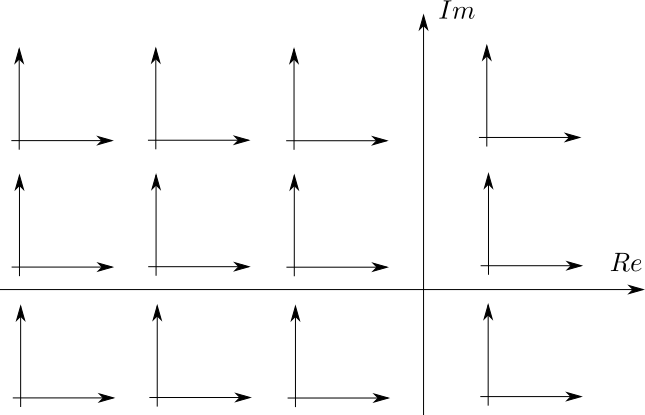
\includegraphics[scale=0.4]{lecture3_fig5.png}

}

\section{\sectiontitleII }
\frame{
\frametitle{Along a Vertical Line}
 	
	As the root moves along a vertical line...\vspc
	
\includegraphics[scale=0.5]{lecture3_fig2.png}

}

\section{\sectiontitleIII }
\frame{
\frametitle{Along a Horizontal Line}
 	
	As the root moves along a horizontal line...\vspc
	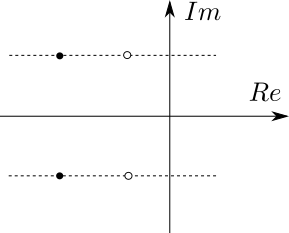
\includegraphics[scale=0.5]{lecture3_fig3.png}

}
\section{\sectiontitleIV }
\frame{
\frametitle{Along a Diagonal Line}
 	
	As the root moves along a diagonal line...\vspc
	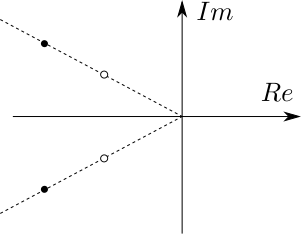
\includegraphics[scale=0.5]{lecture3_fig4.png}

What about the angle of this line?
}

\end{document}









 